%!TEX root=../document.tex

\section{Ergebnisse}

\subsection{Installation und Inbetriebnahme}
Die Installation des Couchbase-Servers wurde auf einem Klon der zur Verfügung gestellten Debian-Testing-VM durchgeführt.

\subsubsection{Installation}
Durchgeführte Schritte:
\begin{enumerate}
	\item Verbinden auf VM mittels SSH
	\item Herunterladen des Couchbase Servers, Community Edition, Version 4.0.0 \cite{couchbase-download}\\
	\texttt{wget http://packages.couchbase.com/releases/4.0.0/couchbase-server-community\\\_4.0.0-debian7\_amd64.deb}
	\item Installation des .deb-Paketes\\
	\texttt{dpkg -i couchbase-server-community\_4.0.0-debian7\_amd64.deb}
	\item Konfiguration des Couchbase-Servers über das Webinterface, erreichbar unter\\
	\texttt{debianvm\_hostname:8091}
\end{enumerate}

\subsubsection{Konfiguration über das Webinterface}
Wie bereits erwähnt, verfügt Couchbase über ein Webinterface. Dieses dient zur Konfiguration sowie auch Verwaltung des Clusters (in Couchbase muss jeder Server einem Cluster zugeordnet sein, auch wenn es nur einen einzelnen Server gibt). Es ist über den Port 8091 erreichbar.

Sobald man zum ersten Mal auf das Webinterface zugreift wird, durchläuft man den Prozess der initialen Konfiguration. Hier müssen diverse Parameter z.B. Benutzername und Passwort des Administrators, RAM pro Node, usw.
Als ,,\textit{Node}'' werden die einzelnen Server innerhalb eines Clusters bezeichnet.

\begin{figure}[!h]
	\begin{center}
		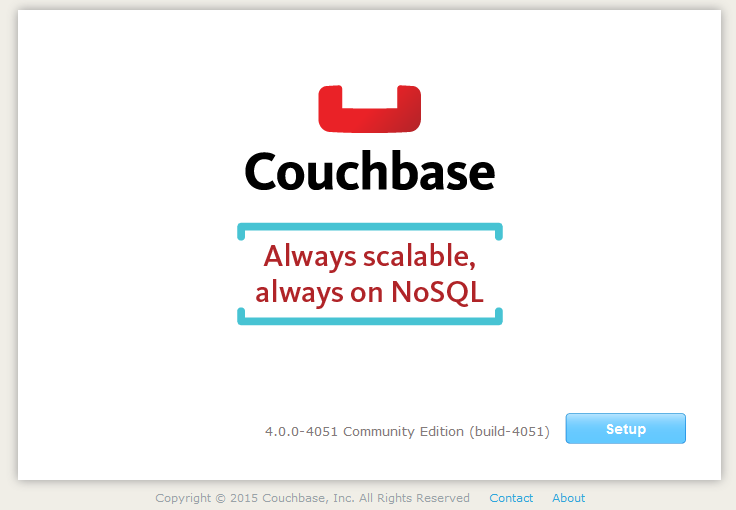
\includegraphics[width=0.5\linewidth]{images/hello-msg.png}
		\caption{,,Startseite'', die beim ersten Aufruf angezeigt wird}
	\end{center}
\end{figure}
\pagebreak
Die Konfiguration wird durch den Button ,,Setup`` auf der Startseite gestartet.

\begin{figure}[!h]
	\begin{center}
		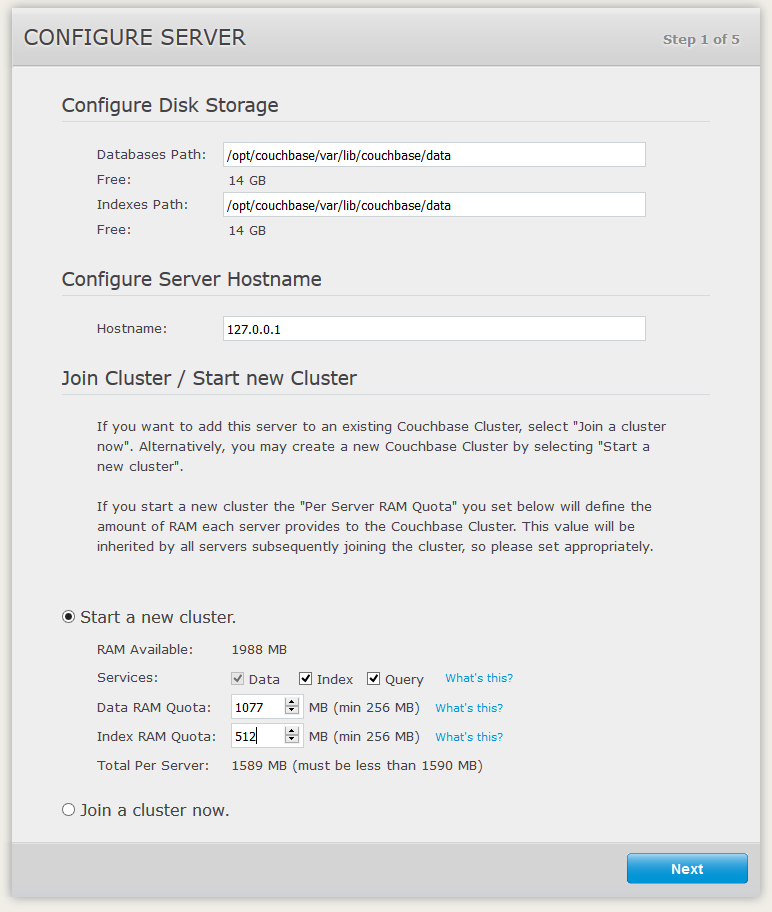
\includegraphics[width=0.6\linewidth]{images/init-config-1.png}
		\caption{Konfiguration der Speicherorte (Pfade), des Hostnames und des Clusters}
	\end{center}
\end{figure}

Im ersten Schritt müssen die Pfade zu den Speicherorten der Datenbank und des Indexes, der Hostname angegeben werden. Weiters muss eingestellt werden, ob dieser Server zu einem bereits bestehenden Cluster hinzugefügt, oder ein neuer Cluster gestartet werden soll.

Hier wird ein neuer Cluster gestartet, muss eingestellt werden, wie viel RAM auf jedem einzelnen Node dieses Clusters von Couchbase (wie viel für Daten, wie viel für den Index) verwendet wird. Es sollte ein Wert eingestellt werden, den alle Nodes unterstützen. Es werden alle Services gewählt, da dieser Node (es wird momentan davon ausgegangen, dass nur ein Node in diesem Cluster existiert) für alle Services zuständig sein soll. In einer Produktionsumgebung ist diese Einstellung jedoch nicht ratsam.

Wenn man einem bestehenden Cluster beitritt, muss man dessen IP-Adresse/Hostname, den Benutzernamen und Passwort des Couchbase Server Administrators, der diesen Cluster verwaltet und die von diesem (neue hinzugefügten) Node zu übernehmenden Services angeben. \cite{couchbase-init-config}

\begin{figure}[!h]
	\begin{center}
		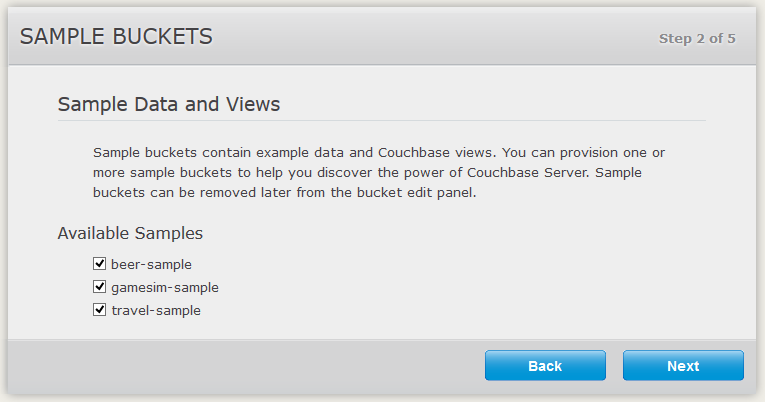
\includegraphics[width=0.7\linewidth]{images/init-config-2.png}
		\caption{Import der Beispieldaten} 
	\end{center}
\end{figure}

In diesem Schritt kann lediglich eingestellt werden ob und welche Beispieldaten importiert werden sollen. Die Rede ist von \textit{Sample Bucket}s. Ein Bucket enthält Dokumente, er entspricht einer Datenbank in einem RDBMS.

Da dies eine Einführung in Couchbase ist, werden alle Sample Buckets aktiviert.
\pagebreak

\begin{figure}[!h]
	\begin{center}
		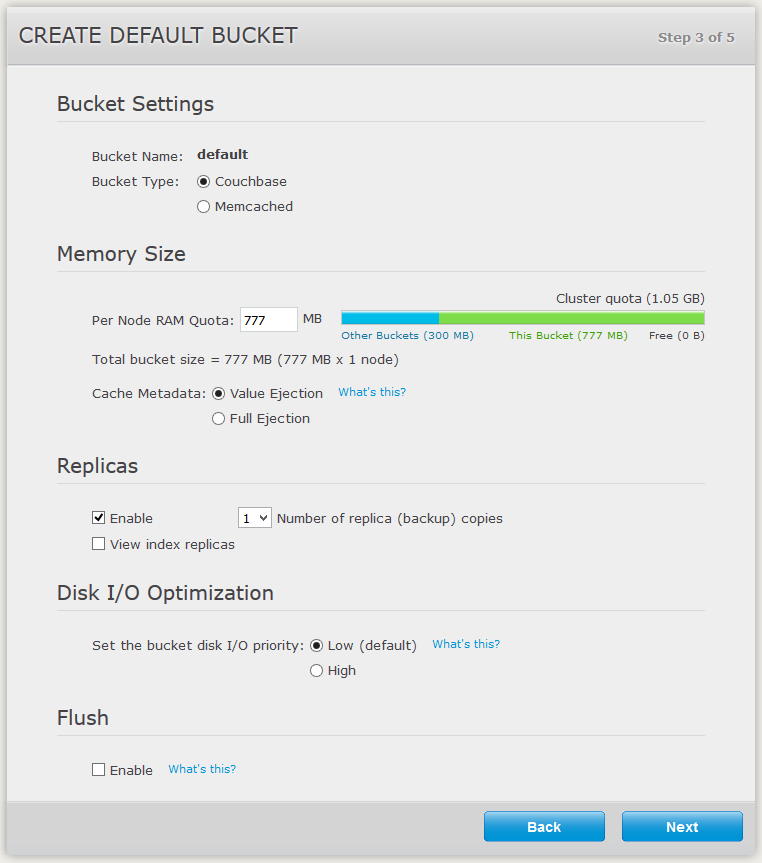
\includegraphics[width=0.7\linewidth]{images/init-config-3.png}
		\caption{Konfiguration des \textit{Default Bucket}s}
	\end{center}
\end{figure}

Im dritten Schritt wird der \textit{Default Bucket} erstellt, dieselbe Seite wird auch für die nachträgliche Erstellung eines Buckets verwendet.

Es können folgende Dinge eingestellt werden \cite{couchbase-new-bucket}:
\begin{itemize}
	\item \textit{Bucket Name}: Normalerweise kann man den Namen des Buckets setzen, da es sich um den Default Bucket handelt, geht das hier \textit{nicht}.
	\item \textit{Bucket Type}: Typ des Buckets, siehe \ref{bucket-types}
	\item \textit{Per Node RAM Quota}: Wie viel RAM für von jedem Node in diesem Cluster (von dem RAM, der Couchbase laut Data RAM Quota (clusterweite Einstellung) auf einem Node zusteht) für diesen Bucket verwendet wird.
	\item \textit{Cache Metadata}: Auswahl der Ejection Policy, siehe \ref{ejection-policy}
	\item \textit{Replicas}: Auswahl, ob dieses Bucket repliziert werden soll. Die Zahl gibt dabei an, auf wie viele andere Nodes repliziert werden soll. Ob die Indizes Views auch repliziert werden sollen kann man ebenfalls auswählen.
	\item \textit{Disk I/O Optimization}: Auswahl der Couchbase-internen Priorität der Zuweisung von Ressourcen zu diesem Bucket auf einem einzelnen Node; funktioniert nur, wenn es mehrere Buckets gibt, die nicht dieselbe Priorität haben (bspw. würde es nicht bringen, wenn alle Buckets die Priorität ,,hoch'' zugewiesen wird)
	\item \textit{Flush}: Durch einen Flush werden alle Objekte in einem Bucket gelöscht. Die Möglichkeit, diese Operation an dem zu erstellenden Bucket durchzuführen, kann hier aktiviert oder deaktiviert werden. In einem memcached-Bucket werden die Objekte nur zum Löschen markiert (,,flag''), in einem Couchbase-Bucket hingegen sofort gelöscht. Diese Option sollte mit großer Vorsicht eingesetzt werden.
	\item (\textit{Auto-Compaction}: Diese Option gibt es nur bei der nachträglichen Erstellung eines neuen Buckets. Dadurch kann die Cluster-weite Auto-Compaction-Konfiguration geändert werden. Es wird empfohlen, diese Einstellung nie zu verwenden.)
\end{itemize}

\begin{figure}[!h]
	\begin{center}
		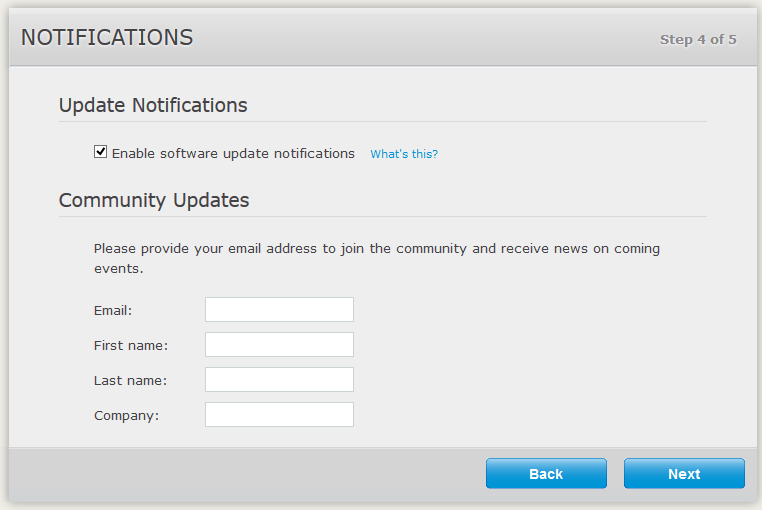
\includegraphics[width=0.7\linewidth]{images/init-config-4.png}
		\caption{Konfiguration der Benachrichtigungen}
	\end{center}
\end{figure}

In Schritt vier kann man angeben, ob man über Software Updates benachrichtigt werden will und sich in der Couchbase Community Mailing List eintragen (um dadurch E-Mails zu Neuigkeiten und Updates zu erhalten).

\begin{figure}[!h]
	\begin{center}
		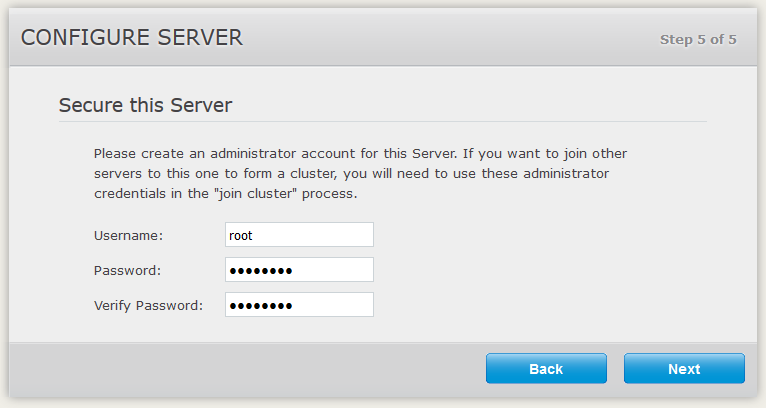
\includegraphics[width=0.7\linewidth]{images/init-config-5.png}
		\caption{Konfiguration der Benachrichtigungen}
	\end{center}
\end{figure}
\pagebreak
Im fünften und letzten Schritt muss man den Benutzernamen und das Passwort des Administrators des Couchbase Servers angeben. Diese Daten werden später bspw. zum Beitritt zu dem Cluster benötigt.

Damit ist das Setup abgeschlossen und der Server zum Betrieb bereit.

\subsubsection{Bucket-Typen}
\label{bucket-types}
Es gibt zwei Typen von Buckets:
\begin{itemize}
	\item \textit{Couchbase}
	\item \textit{memcached}
\end{itemize}
Ein Couchbase-Bucket ist im Prinzip eine verteilte Datenbank, also genau das, was man erwarten würde. Dieser Bucket-Typ unterstützt Caching, Persistierung, Replikation von Daten sowie auch die Lastverteilung und das dynamische Hinzufügen und Entfernen von Servern in diesem Cluster.

Ein memcached-Bucket ist ein verteilter Key-Value-Cache. Alle Datensätze befinden sich dabei also nur im Cache. Sobald kein RAM mehr zur Verfügung steht, werden Datensätze nach dem LRU (,,Least Recently Used'')-Algorithmus entfernt. Diese entfernten Datensätze können nicht wiederhergestellt werden! Memcached-Buckets sind für die Verwendung neben anderen Systemen entworfen und gedacht. \cite{couchbase-buckets}

\subsubsection{Ejection Policy}
\label{ejection-policy}
Wie der Cache eines Buckets geleert wird, kann durch die \textit{Ejection Policy} (,,Auswerf-Strategie'') festgelegt werden. Dabei gibt es zwei Möglichkeiten \cite{couchbase-database-engine-architecture}:
\begin{itemize}
	\item \textit{Value-only Ejection} (default))\\
	Daten werden aus dem Cache entfernt, jedoch bleiben alle Keys und Metadaten (auch für gelöschte Einträge) vorhanden. Diese Einstellung wird besonders in Fällen gebraucht, wenn eine kleine Latenzzeit von großer Bedeutung ist (und der RAM des Clusters ausreichend groß ist).
	\item \textit{memcached}\\
	Alle Daten werden inklusive der Keys und Metadaten aus dem Cache entfernt. Bei Anwendungsfälle, in denen die Datenmenge sehr groß ist, oder auf ein großer Teil der Daten nur selten zugegriffen wird, von Vorteil. Höhere Latenzzeiten müssen dabei akzeptiert werden.
\end{itemize}

\subsubsection{Webinterface}
Nach Abschluss der Installation und initialen Konfiguration wird das Webinterface angezeigt. Über dieses wird das gesamte Cluster verwaltet: es können zahlreiche Statistiken zur Serverlast eingesehen, Buckets, Dokumente und Views verwaltet, die Konfiguration geändert werden, usw.

\begin{figure}[!h]
	\begin{center}
		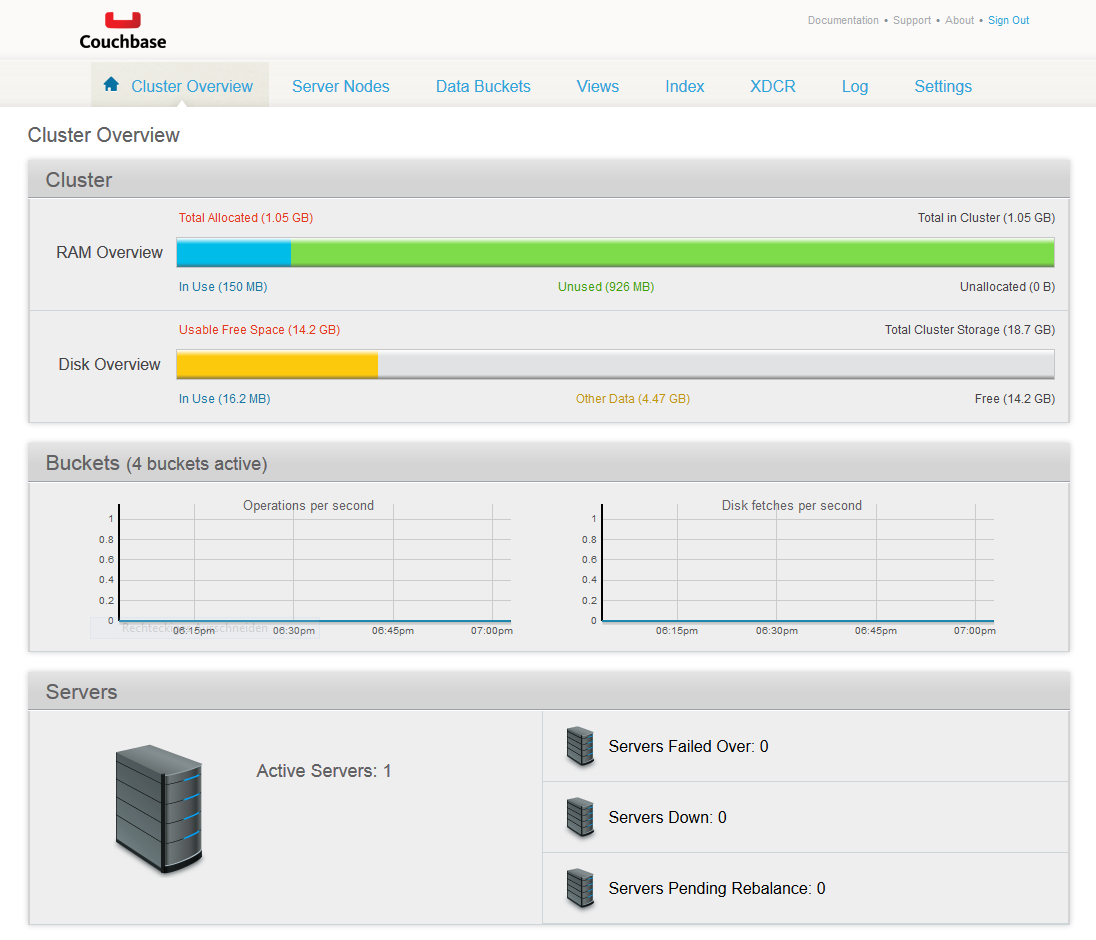
\includegraphics[width=0.7\linewidth]{images/overview.png}
		\caption{Startseite des Webinterfaces}
	\end{center}
\end{figure}

Auf das Webinterface wird nicht weiter eingegangen, da die Verwendung intuitiv ist und andererseits alle möglichen Optionen bereits geklärt wurde, oder noch im Laufe des Protokolls (Durchführung in CLI oder Client-Applikation) noch geklärt werden.

\subsection{Dokumentenstruktur}
In Couchbase können Daten entweder als JSON-Dokumente oder in einem binären Format gespeichert werden. In diesem Kapitel wird nur auf die Dokumente und deren Struktur eingegangen, nicht aber auf JSON selbst oder binäre gespeicherte Daten.

Ein Dokument in Couchbase repräsentiert üblicherweise eine Instanz eines Objektes im Code des Clients. Es ist vergleichbar mit einem Datensatz, einer Zeile in einer Tabelle, in einem RDBMS. Die Attribute des Dokuments sind ähnlich wie die Spalten einer Tabelle in einem RDBMS. Jedoch gibt es kein Schema, dass die Struktur eines Dokumentes vorgibt (wie in RDBMS die Tabelle die Spalten vorgibt), jedes Dokument kann verschiedene Attribute haben. Wenn der Client zwischen verschiedenen Typen unterscheiden muss, kann man bspw. ein Attribut ``Typ'' hinzufügen (Abfrage des Typens in View bietet sich an).

Dokumente können ineinander verschachtelte Strukturen (JSON: Objekte können weitere Objekte enthalten) enthalten (sog. ``Sub-Dokumente''). So können Beziehungen oder Hierarchien natürlicher und kompakter als in einem RDBMS dargestellt werden.

\subsubsection{Praktisches Beispiel des Dokumentenmodels}
Ein Unternehmen möchte eine Online-Flug-Booking-Anwendung, mit der ein User nach Flügen an einem bestimmten Datum suchen kann.

Ein relationales Model für eine Datenbank, welche die Flüge enthält, könnte in etwa so aussehen: Es gibt eine Tabelle für Fluglinien, Flüge und Zeitplan. Jeder Flug ist einer Fluglinie zugeordnet und hat einen Zeitplan (mit Abflugzeit, Ankunftszeit, usw.).

\begin{figure}[!h]
	\begin{center}
		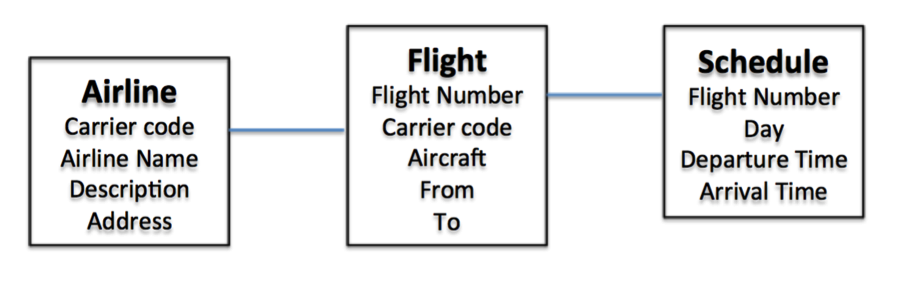
\includegraphics[width=0.4\linewidth]{images/relational-model-flight-status.png}
		\caption{Mögliches Model bei Verwendung einer relationalen Datenbank}
	\end{center}
\end{figure}

In Couchbase hingegen könnt es anders aussehen. Hier könnte es ein Dokument für eine Route geben. Dieses Dokument könnte eine Liste (Array) von Sub-Dokumenten für die einzelnen Flüge und deren Zeitplänen haben.

\begin{figure}[!h]
	\begin{center}
		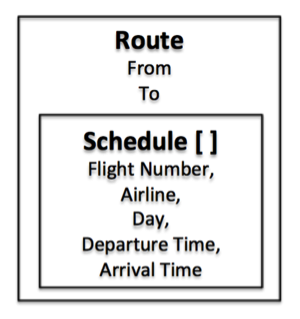
\includegraphics[width=0.15\linewidth]{images/document-data-model-flight-booking.png}
		\caption{Mögliches Model bei Verwendung von Couchbase}
	\end{center}
\end{figure}

\subsubsection{Dynamisches Schema}

\subsubsection{Designentscheidungen für Dokumente}

\subsection{Indizierung und Map/Reduce}
Ein Index ist eine Liste von Daten die das Durchsuchen von Dokumenten effizienter macht. Dadurch müssen nicht mehr alle einzelnen Dokumente durchsucht werden, sondern es können 	
Eine Map/Reduce-View (oder auch nur View) erstellt einen angepassten Index, je nach Abfrage der View. So eine View besteht aus JavaScript-Funktionen (\texttt{map} und \texttt{reduce}), die mit Dokumenten eines DataBucket arbeiten.

Views sind ausgewählte Daten aus Dokumenten. Eine View durchsucht ein DataBucket und speichert jene Informationen die in der View angegeben sind in einem Index. Dabei gibt es 2 Arten von Views:
\begin{itemize}
	\item Bei einer Development View wird nur ein Subset (d.h. ein kleiner Teil) des Ergebnisses indiziert. 
	\item Bei einer Production View werden alle Ergebnisse zum dem Index hinzugefügt.
\end{itemize}

Das Ergebnis einer View kann über die Reduce-Funktion zusammengefasst bzw. ,,reduziert`` werden. Die Reduce Funktion ist eine optionale Funktion der View und kann über Funktionen (z.B. count, sum,..) Ergebnisse auf genau einen Wert reduzieren. 

In Couchbase können auch eigene Reduce-Funktionen verwendet werden. Dabei ist zu beachten, dass eine Reduce-Funktion aus mehreren sogenannten \textit{Rereduce}-Funktionen besteht. Die Ergebnisse der Map-Funktion werden in mehrere ,,Gruppen`` eingeteilt. Auf diese einzelnen Gruppen wird anschließend die Reduce-Funktion angewandt und die Ergebnisse in einem B-Baum gespeichert. Dieser Vorgang wird solange wiederholt, bis ein einzelnes Ergebnis vorhanden ist.

Falls ein Dokument, auf das sich eine Abfrage bezieht, ändert bzw. eine neues Dokument hinzugefügt wird, muss dieses neu indiziert werden. Dabei gibt es 3 Möglichkeiten:
\begin{itemize}
	\item Es wird sofort zum Index hinzugefügt (nicht empfehlenswert wegen Performanceverlust)
	\item Es wird vor der nächsten Abfrage zum Index hinzugefügt
	\item Wenn der Cluster unausgelastet ist, jedoch vor der nächsten Abfrage
\end{itemize}

Neben einer Map/Reduce-View gibt es auch andere Views, die Indizes erzeugen:
\begin{itemize}
	\item Spatial Views\\
	Spatial Views enthalten nur eine Funktion (ähnlich mit der Map Funktion) und sind für geometrisch bzw. räumliche Abfragen.
	\item Global Secondary Index
	Ein Global Secondary Index (GIS) erzeugt Indizes von einem gesamten Cluster.
\end{itemize}

\subsection{CLI-Befehle}

\subsection{Client-API-Installation und Verwendung}
\subsubsection{Installation}
Die Java-Client-API kann von http://developer.couchbase.com/documentation/server/4.1/sdks/java-2.2/download-links.html heruntergeladen werden. Die JARs müssen im Build-Path eingebunden werden. Die Bibliotheken sind auch in einem Maven Repository verfügbar, könnten also einfach als Abhängigkeiten in der \texttt{pom.xml} eingetragen werden.
\subsubsection{Verbindungsaufbau (Connection)}
Die grundsätzliche Verbindung zu einem Couchbase Cluster erfolgt über die Klasse \texttt{CouchbaseCluster}. Es muss nur ein Teil der Nodes des Clusters übergeben werden, da die eigentliche Verbindung (also das Erstellen des Sockets) erst hergestellt wird, wenn man sich zu einem DataBucket verbindet. Die Verbindung wird in einem Cluster-Objekt gespeichert und kann über dieses verwaltet werden.
%todo code snippet connect
Mit \texttt{cluster.openBucket()} wird eine Verbindung zu einem DataBucket hergestellt (es können Name des Buckets, eventuell Passwort und die Timeout-Zeit übergeben werden, ohne Parameter wird das default-Bucket verwendet).

Über \texttt{cluster.disconnect()} werden die Verbindungen zu den Buckets sowie zu dem Cluster geschlossen.

%todo code snippet disconnect

\subsubsection{CRUD (auf Dokumente)}

\paragraph{Create}\hspace{0pt}\\
Dokumente können im \texttt{JSONDocument}-Format in einen Bucket eingefügt werden. Ein \texttt{JSONDocument} besteht aus \texttt{JSONObject}s (bzw. ein JSONObjects-Array). In einem Dokument werden zusätzlich noch Meta-Daten (wie ID, Ablaufzeit, CAS-Value,...) gespeichert. Ein JSONDocument wird über \texttt{JsonDocument.create} erstellt, wobei ID und Inhalt (also das \texttt{JSONObject}) übergeben werden.
%todo code snippet document create
Das Dokument kann über \texttt{bucket.upsert} oder \texttt{bucket.insert} eingefügt werden. \textit{Upsert} überschreibt ein eventuell vorhandenes Dokument (kann somit auch für ,,Update'' verwendet werden). \textit{Insert} speichert das Dokument, wirft jedoch eine \texttt{DocumentAlreadyExistsException} falls das Dokument schon existiert.

\paragraph{Read}\hspace{0pt}\\
Ein Dokument kann über \texttt{bucket.get(id)} (null falls das Dokument nicht gefunden wurde) gelesen werden. Das gelesene Dokument wird in einem \texttt{JSONDocument}-Objekt gespeichert. 
Über \texttt{JSONDocument.Content().get()} können Daten aus dem Dokument ausgelesen werden. 
Über \texttt{bucket.getAndLock(id, locktime)} kann ein Dokument für Schreibzugriffe gesperrt werden (nicht für Lesezugriffe). Ein Dokument kann für maximal 30 Sekunden gelockt werden (15 Sekunden per default) und kann über \texttt{unlock()} (frühzeitig) wieder freigegeben werden.
Über \texttt{bucket.getAndTouch(id, expiryTime)} wird die Ablaufzeit erneuert werden (funktioniert auch mit nur \texttt{touch()} falls nur Ablaufzeit erneuert werden soll). 

\subsubsection{Views}


\subsection{GitHub}
Repository: \href{https://github.com/pkomon-tgm/Couchbase-Protocol}{https://github.com/pkomon-tgm/Couchbase-Protocol}
\subsection{Zeitschätzung}
\renewcommand{\arraystretch}{1.5}
\begin{table}[!h]
	\center
	\begin{tabular}{ | @{\hspace{3mm}} c @{\hspace{3mm}} | @{\hspace{3mm}} l @{\hspace{3mm}} | c |}
		\hline Arbeit & geschätzter Zeitaufwand & tatsächlicher Zeitaufwand\\ \hline\hline
		Installation & 0,5h & \\ \hline
		CLI-Client installieren und testen & 1h & \\ \hline
		API-Installation und Verwendung & 1h &\\ \hline
		Views erstellen und testen & 2h & \\ \hline
		Recherche und Protokoll schreiben & 4h & \\ \hline
	\end{tabular}
\end{table}
